	% \documentclass[12pt]{article}

%%v helpful MIT exam schema, see http://www-math.mit.edu/~psh/exam/examdoc.pdf
 \documentclass[12pt]{exam} 
% \qformat{\textbf{Question \thequestion}\quad \thepoints\hfill } % Large depth to make space}
 \renewcommand{\thesubpart}{(\roman{subpart})}
 \renewcommand{\subpartlabel}{\thesubpart}
% \footer{}{}{Page \thepage\ de \numpages}
\addpoints
\pointsinmargin
% \boxedpoints
\renewcommand{\questionshook}{\setlength{\itemsep}{2mm}}
\renewcommand{\partshook}{
	\setlength{\itemsep}{15mm}
}

\usepackage{cmbright}

\pagestyle{empty} %for handouts
\addtolength{\jot}{2em} % this makes all formulae a bit more spaced vertically for handouts
\setlength{\parindent}{0pt} %we're not writing a novel
\renewcommand{\arraystretch}{1.5} %makes tables taller, so easier to write in

\usepackage[fleqn]{amsmath}
\usepackage{amssymb} %standard classy maths symbols
\usepackage[a4paper, margin=1in]{geometry} %makes it easy to specify where to put stuff on the page

\usepackage{siunitx} %v handy way of getting SI units to typeset correctly...
% \sisetup{locale = FR} %... and now it will use a comma for decimals

\usepackage[utf8]{inputenc}

% \usepackage[french]{babel} % frenchify everything (e.g. a Table becomes a Tableau)
% \usepackage{lmodern} % font with nicer French characters than standard
% \usepackage{textcomp} % and more help for special characters

\usepackage{tcolorbox} % basic but good package for boxes around text
\tcbset{colback=black!5!white}
% \usepackage{color} % colours
%\newcommand{\fillin}{\color{black!1!white}} %makes the text disappear
%\definecolor{fillin}{rgb} {1.00,1.00,1.00}
%\renewcommand{\fillin}{\color{blue}} \definecolor{fillin}{rgb} {0.00,0.00,1.00} %makes the filling in text appear (in blue)

\usepackage{enumitem} % can change the labels on lists, items, enumerates
\usepackage{setspace}

\usepackage{tikz, tkz-euclide} % interval diagrams, sets, etc.
%\usetikzlibrary{calc,trees,positioning,arrows,fit,shapes}

\begin{document}

\textbf{Name:} \dotfill

\
\begin{questions}


\question[2] Take a \textbf{triangle} with sidelengths $a < b < c$. In order to apply \textbf{Pythagoras' Theorem}, we must check that the triangle is...
\fillwithdottedlines{7mm}
If this hypothesis is true, then we can conclude what \textbf{equation} relating $a$, $b$ and $c$ ?
\fillwithdottedlines{7mm}

\question[4] Find the area of this isosceles triangle with perimeter 12cm.
\vspace{-5mm}

\begin{minipage}{0.8\textwidth}
\vspace{3mm}
\fillwithdottedlines{55mm}
\end{minipage}
\begin{minipage}{0.2\textwidth}
\begin{center}

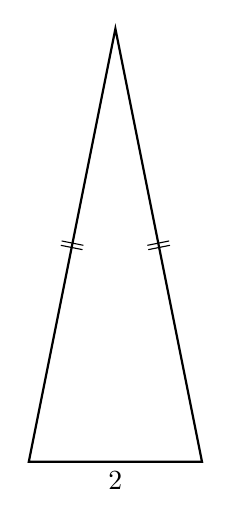
\begin{tikzpicture}[scale=1.1]
\coordinate (A) at (-1,0);
\coordinate (B) at (1,0);
\coordinate (C) at (0,5);

\draw[thick] (A)-- node[below] {2} (B)--  (C)--cycle;
\tkzMarkSegment[pos=.5,mark=||](B,C) 
\tkzMarkSegment[pos=.5,mark=||](A,C) 

\end{tikzpicture}



\end{center}
\end{minipage}

\question[3] These two \textbf{triangles} are \textbf{similar}. Find the named lengths.
\vspace{-3mm}

\begin{center}
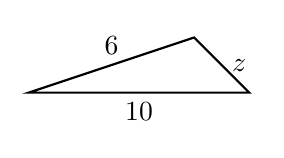
\begin{tikzpicture}[scale= 0.7]
\draw[thick] (0,0) -- node[below] {10} (4,0) -- node[right] {$z$} (3,1) -- node[above] {6} cycle;
\end{tikzpicture}
\hspace{10mm}
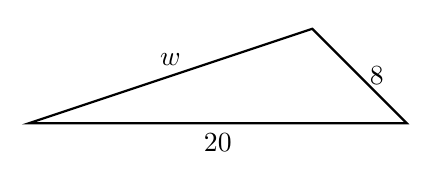
\begin{tikzpicture}[scale= 1.2]
\draw[thick] (0,0) -- node[below] {20} (4,0) -- node[right] {8} (3,1) -- node[above] {$w$} cycle;
\end{tikzpicture}
\end{center}
\vspace{-4mm}
\fillwithdottedlines{21mm}


\vfill

\question \textbf{Bonus.} 
What is the shaded area of this square? \hfill \emph{Work on the back.}
\vspace{-2mm}

\begin{center}

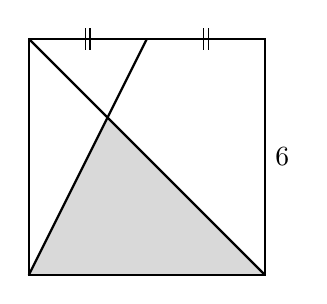
\begin{tikzpicture}
\coordinate (O) at (0,0);
\coordinate (A) at (3,0);
\coordinate (B) at (3,3);
\coordinate (C) at (1.5,3);
\coordinate (D) at (0,3);

\fill[black!15] (O)  -- (1, 2) -- (A) -- cycle;
\draw[thick] (O)-- (A)-- node[right] {6} (B)--(D)--cycle;
\draw[thick] (O)--(C);
\draw[thick] (A)--(D);
\tkzMarkSegment[pos=.5,mark=||](B,C) 
\tkzMarkSegment[pos=.5,mark=||](C,D) 

\end{tikzpicture}
\end{center}


\end{questions}

\begin{tcolorbox}

\textbf{Name of the person marking:}

\begin{center}
\gradetable[h][questions]
\end{center}

\end{tcolorbox}

\end{document}